

\subsection{LI-rezoluce}

V obecném lineárním důkazu může být každá následující boční klauzule buď axiom z $S$ nebo jedna z předchozích centrálních klauzulí. Pokud zakážeme druhou možnost, budeme-li tedy požadovat, aby všechny boční klauzule byly z $S$, dostaneme tzv. \emph{LI (linear-input)} rezoluci:
    
\begin{definition}[LI-důkaz]
    \emph{LI-důkaz} (rezolucí) klauzule $C$ z formule $S$ je lineární důkaz 
    $$
    \begin{bmatrix}
        C_0 \\
        B_0
    \end{bmatrix},
    \begin{bmatrix}
        C_1 \\
        B_1
    \end{bmatrix},\dots,
    \begin{bmatrix}
        C_n \\
        B_n
    \end{bmatrix},
    C
    $$
    ve kterém je každá boční klauzule $B_i$ axiom z $S$. Pokud LI-důkaz existuje, říkáme, že je $C$ \emph{LI-dokazatelná} z $S$, a píšeme $S\proves_{LI}C$. Pokud $S\proves_{LI}\square$, je $S$ \emph{LI-zamítnutelná}.
\end{definition}

\begin{remark}
    LI-důkaz přímo dává rezoluční strom (všechny listy jsou axiomy), a to ve speciálním tvaru, kterému bychom mohli říkat `chlupatá cesta'. A naopak, z rezolučního stromu ve tvaru chlupaté cesty okamžitě získáme LI-důkaz: vrcholy na cestě jsou centrální klauzule, chlupy jsou boční klauzule.
\end{remark}

Zatímco \emph{lineární rezoluce}\footnote{Tj. dokazovací systém založený na hledání \emph{lineárních} důkazů resp. zamítnutí.} je jen jiný pohled na obecný rezoluční důkaz, \emph{LI-rezoluce} přináší zásadní omezení: ztrácíme \emph{úplnost} (ne každá nesplnitelná formule má LI-zamítnutí). Na druhou stranu, LI-důkazy je jednodušší konstruovat.\footnote{V každém kroku máme k volbě jen klauzule z $S$, nikoliv předchozí dokázané centrální klauzule.} 

\subsection{Úplnost LI-rezoluce pro Hornovy formule}

Jak si nyní ukážeme, LI-rezoluce je \emph{úplná pro Hornovy formule}. A jak uvidíme v následující sekci, je základem interpreterů jazyka Prolog, který s Hornovými formulemi pracuje. Nejprve připomeňme terminologii týkající se hornovskosti a také programů, a to v množinové reprezentaci:

\begin{itemize}
    \item \emph{Hornova klauzule} je klauzule obsahující nejvýše jeden pozitivní literál.
    \item \emph{Hornova formule} je (konečná, nebo i nekonečná) množina Hornových klauzulí.
    \item \emph{Fakt} je pozitivní jednotková (Hornova) klauzule, tj. $\{p\}$, kde $p$ je výroková proměnná.
    \item \emph{Pravidlo} je (Hornova) klauzule s právě jedním pozitivním a alespoň jedním negativním literálem.
    \item Pravidlům a faktům říkáme \emph{programové klauzule}.
    \item \emph{Cíl} je neprázdná (Hornova) klauzule bez pozitivního literálu.\footnote{Připomeňme, že dokazujeme \emph{sporem}, tedy \emph{cíl} je negací toho, co bychom chtěli dokázat.}
\end{itemize}

Bude se nám hodit následující jednoduché pozorování:

\begin{observation}\label{observation:horn-fact-goal}
    Je-li Hornova formule $S$ nesplnitelná a $\square\notin S$, potom obsahuje fakt i cíl.
\end{observation}
\begin{proof}
    Neobsahuje-li fakt, můžeme ohodnotit všechny proměnné 0; neobsahuje-li cíl, ohodnotíme 1.
\end{proof}

Nyní vyslovíme a dokážeme Větu o úplnosti LI-rezoluce pro Hornovské formule. Důkaz dává také návod, jak LI-zamítnutí zkonstruovat, a to na základě průběhu jednotkové propagace. Tento postup ilustrujeme na příkladu níže, který můžete sledovat souběžně s čtením důkazu.

\begin{theorem}[O úplnosti LI-rezoluce pro Hornovy formule]\label{theorem:completeness-of-li-resolution-for-horn}
Je-li Hornova formule $T$ splnitelná, a $T\cup\{G\}$ je nesplnitelná pro cíl $G$, potom $T\cup\{G\}\proves_{LI}\square$, a to LI-zamítnutím, které začíná cílem $G$.   
\end{theorem}
\begin{proof}
    Podobně jako ve Větě o úplnosti rezoluce můžeme díky Větě o kompaktnosti předpokládat, že $T$ je konečná. Důkaz (konstrukci LI-zamítnutí) provedeme indukcí podle počtu proměnných v $T$.

    Z Pozorování \ref{observation:horn-fact-goal} plyne, že $T$ obsahuje fakt $\{p\}$ pro nějakou výrokovou proměnnou $p$. Protože $T\cup\{G\}$ je nesplnitelná, je podle Lemmatu \ref{lemma:tree-of-reductions} nesplnitelná také $(T\cup\{G\})^p=T^p\cup\{G^p\}$, kde $G^p=G\setminus\{\neg p\}$.
    
    Pokud $G^p=\square$, potom $G=\{\neg p\}$, $\square$ je rezolventa $G$ a $\{p\}\in T$, a máme jednokrokové LI-zamítnutí $T$ (to je báze indukce). 
    
    Jinak je formule $T^p$ splnitelná (stejným ohodnocením jako $T$, neboť to musí obsahovat $p$ kvůli faktu $\{p\}$, tedy neobsahuje $\neg p$) a má méně proměnných než $T$. Tedy podle indukčního předpokladu existuje LI-odvození $\square$ z $T^p\cup\{G^p\}$ začínající $G^p=G\setminus\{\neg p\}$.

    Hledané LI-zamítnutí $T\cup\{G\}$ začínající $G$ zkonstruujeme (podobně jako v důkazu Věty o úplnosti rezoluce) přidáním literálu $\neg p$ do všech listů, které už nejsou v $T\cup\{G\}$ (tedy vznikly odebráním $\neg p$), a do všech vrcholů nad nimi. Tím získáme $T\cup\{G\}\proves_{LI}\neg p$, na závěr přidáme boční klauzuli $\{p\}$ a odvodíme $\square$.
\end{proof}
%todo: another potential frozen bucket, restructure the induction proof?

\begin{example}\label{example:linear-input-resolution}
Mějme (splnitelnou, hornovskou) teorii $T$, kterou zapíšeme v množinové reprezentaci jako formuli $T=\{\{p,\neg r,\neg s\},\{\neg q,r\},\{q,\neg s\},\{s\}\}$. Představte si, že chceme dokázat, že v teorii $T$ platí $p\land q$.\footnote{Tj. v Prologu bychom položili `dotaz' (`query'): \texttt{?-p,q.}} V rezoluční metodě uvážíme cíl $G=\{\neg p,\neg q\}$ a ukážeme, že $T\cup\{G\}\proves_{LI}\square$. 

Dle návodu z důkazu najdeme ve formuli $T$ fakt, a provedeme pomocí něho jednotkovou propagaci v $T$ i v cíli $G$. Postup opakujeme, dokud není formule prázdná:
\begin{itemize}
    \item $T=\{\{p,\neg r,\neg s\},\{\neg q,r\},\{q,\neg s\},\{s\}\}$, $G=\{\neg p,\neg q\}$
    \item $T^s=\{\{p,\neg r\},\{\neg q,r\},\{q\}\}$, $G^s=\{\neg p,\neg q\}$
    \item $T^{sq}=\{\{p,\neg r\},\{r\}\}$, $G^{sq}=\{\neg p\}$
    \item $T^{sqr}=\{\{p\}\}$, $G^{sqr}=\{\neg p\}$
    \item $T^{sqrp}=\emptyset$, $G^{sqrp}=\square$
\end{itemize}
Nyní zpětným postupem sestrojíme rezoluční zamítnutí:
\begin{itemize}
    \item $T^{sqrp},G^{sqrp}\proves_{LI}\square$:
    \begin{center}
        \begin{forest}
            for tree={math content,grow=west,text height=2ex, text depth=1ex, l sep=3em}
                        [{\square}]                       ]
        \end{forest} 
    \end{center}
    \item $T^{sqr},G^{sqr}\proves_{LI}\square$:
    \begin{center}
        \begin{forest}
            for tree={math content,grow=west,text height=2ex, text depth=1ex, l sep=3em}
                        [{\square}
                            [,phantom]
                            [{\{\neg p\}}]
                            [{\{p\}}]                        
                        ]
        \end{forest} 
    \end{center}
    
    \item $T^{sq},G^{sq}\proves_{LI}\square$:
    \begin{center}
        \begin{forest}
            for tree={math content,grow=west,text height=2ex, text depth=1ex, l sep=3em}
                    [{\square}
                        [,phantom]
                        [{\{\neg r\}}
                            [,phantom]
                            [{\{\neg p\}}]
                            [{\{p,\neg r\}}]                        
                        ]
                        [{\{r\}}]
                    ]
        \end{forest} 
    \end{center}
    
    \item $T^{s},G^{s}\proves_{LI}\square$:
    \begin{center}
        \begin{forest}
            for tree={math content,grow=west,text height=2ex, text depth=1ex, l sep=3em}
                [{\square}
                    [,phantom]
                    [{\{\neg q\}}
                        [,phantom]
                        [{\{\neg q,\neg r\}}
                            [,phantom]
                            [{\{\neg p,\neg q\}}]
                            [{\{p,\neg r\}}]                        
                        ]
                        [{\{\neg q,r\}}]
                    ]
                    [{\{q\}}]                    
                ]
        \end{forest} 
    \end{center}
    
    \item $T,G\proves_{LI}\square$
    \begin{center}
        \begin{forest}
            for tree={math content,grow=west,text height=2ex, text depth=1ex, l sep=3em}
            [{\square}
                [,phantom]
                [{\{\neg s\}}
                    [,phantom]
                    [{\{\neg q,\neg s\}}
                        [,phantom]
                        [{\{\neg q,\neg r,\neg s\}}
                            [,phantom]
                            [{\{\neg p,\neg q\}}]
                            [{\{p,\neg r,\neg s\}}]                        
                        ]
                        [{\{\neg q,r\}}]
                    ]
                    [{\{q,\neg s\}}]                    
                ]
                [{\{s\}}]
            ]
        \end{forest}
    \end{center}
\end{itemize}
\end{example}

\section{Rezoluce v Prologu}

Ačkoliv skutečná síla Prologu vychází z tzv. \emph{unifikace} a z rezoluce v predikátové logice, ukážeme si jak Prolog využívá rezoluční metodu na příkladě \emph{výrokového} programu. Adaptace na predikáty bude později přímočará.

\subsection{Program v Prologu}

\emph{Program} v Prologu je Hornova formule obsahující pouze \emph{programové klauzule}, tj. \emph{fakta} nebo \emph{pravidla}. \emph{Dotaz} je konjunkce faktů, negace dotazu je \emph{cíl}.

\begin{example}
Jako příklad programu v Prologu využijeme teorii (formuli) $T$ a dotaz $p\land q$ z Příkladu \ref{example:linear-input-resolution}. Například klauzuli $\{p,\neg r,\neg s\}$, která je ekvivalentní $r\land s\limplies p$, zapíšeme v Prologu jako: \texttt{p:-r,s.}
\begin{verbatim}
    p:-r,s.
    r:-q.
    q:-s.
    s.    
\end{verbatim}
A programu položíme dotaz:
\begin{verbatim}
    ?-p,q.    
\end{verbatim}
\end{example}

\begin{corollary}
    Mějme program $P$ a dotaz $Q=p_1\land\dots\land p_n$, a označme $G=\{\neg p_1,\dots,\neg p_n\}$ (tj. $G\sim \neg Q$). Následující podmínky jsou ekvivalentní:
    \begin{itemize}
        \item $P\models Q$,
        \item $P\cup\{G\}$ je nesplnitelná,
        \item $P\cup\{G\}\proves_{LI}\square$, a existuje LI-zamítnutí začínající cílem $G$.
    \end{itemize}
\end{corollary}
\begin{proof}
    Ekvivalence prvních dvou podmínek je důkaz sporem, ekvivalence druhé a třetí je Věta o úplnosti LI-rezoluce pro Hornovy formule.
\end{proof}

\subsection{(draft) SLD-rezoluce}\todo


% from slides:

\subsubsection*{Rezoluce v Prologu}
\emph{1) S klauzulemi interpret pracuje jako s \myblue{uspořádanými seznamy} literálů.}


\mdef{LD-rezoluce} (\emph{linear definite}) je $LI$-rezoluce, při které v každém kroku rezolventa aktuálního cíle \mygreen{$(\neg p_1, \dots, \neg p_{i-1},\neg p_i, \neg p_{i+1},\dots, \neg p_n)$} a boční
klauzule \mygreen{$(p_i, \neg q_1, \dots, \neg q_m)$} je:
$$(\neg p_1, \dots, \neg p_{i-1},\neg q_1, \dots, \neg q_m, \neg p_{i+1},\dots, \neg p_n)$$

{\bf \myblue{Pozorování}}\ \ {\it Každý LI-důkaz lze transformovat na LD-důkaz stejné klauzule}
{\it ze stejné formule se stejnou počáteční klauzulí (cílem).}

\medskip

\noindent \emph{2) Výběr literálu z cílové klauzule, přes který se rezolvuje, je určen daným}
\emph{\myblue{selekčním pravidlem} $\mathcal{R}$. Typicky, ``vyber první literál z aktuálního cíle''.}

\mdef{SLD-rezoluce} (\emph{selection}) dle $\mathcal{R}$ je $LD$-rezoluce, při které se v kroku $(C_i,B_i)$
rezolvuje přes literál $\mathcal{R}(C_i)$.

\medskip

{\bf \myblue{Pozorování}}\ \ {\it Každý LD-důkaz lze transformovat na SLD-důkaz stejné}
{\it klauzule ze stejné formule se stejnou počáteční klauzulí (cílem).}

\medskip

{\bf \myblue{Důsledek}}\ \ {\it SLD-rezoluce je \myblue{úplná} pro dotazy nad programy v Prologu.}


%%%%%%%%%%%%%%%%%%%%%%%%%%%%%%%%%%%%%%%%%%%%%%%%%%%%%%5

\subsubsection*{Prohledávací SLD-strom}
{\it Dosud není určen výběr programové klauzule pro rezoluci s aktuálním cílem.}

\mdef{SLD-strom} programu $P$ a cíle $G$ pro selekční pravidlo $\mathcal{R}$ je strom s vrcholy označenými cíly takový, že kořen je označen $G$ a je-li nějaký vrchol označen $G'$, má tolik synů, kolik je \myblue{možností} rezolucí $G'$ s programovými klauzulemi v $P$ dle literálu $\mathcal{R}(G')$. Synové jsou označeni příslušnými rezolventami.

\smallskip
\centerline{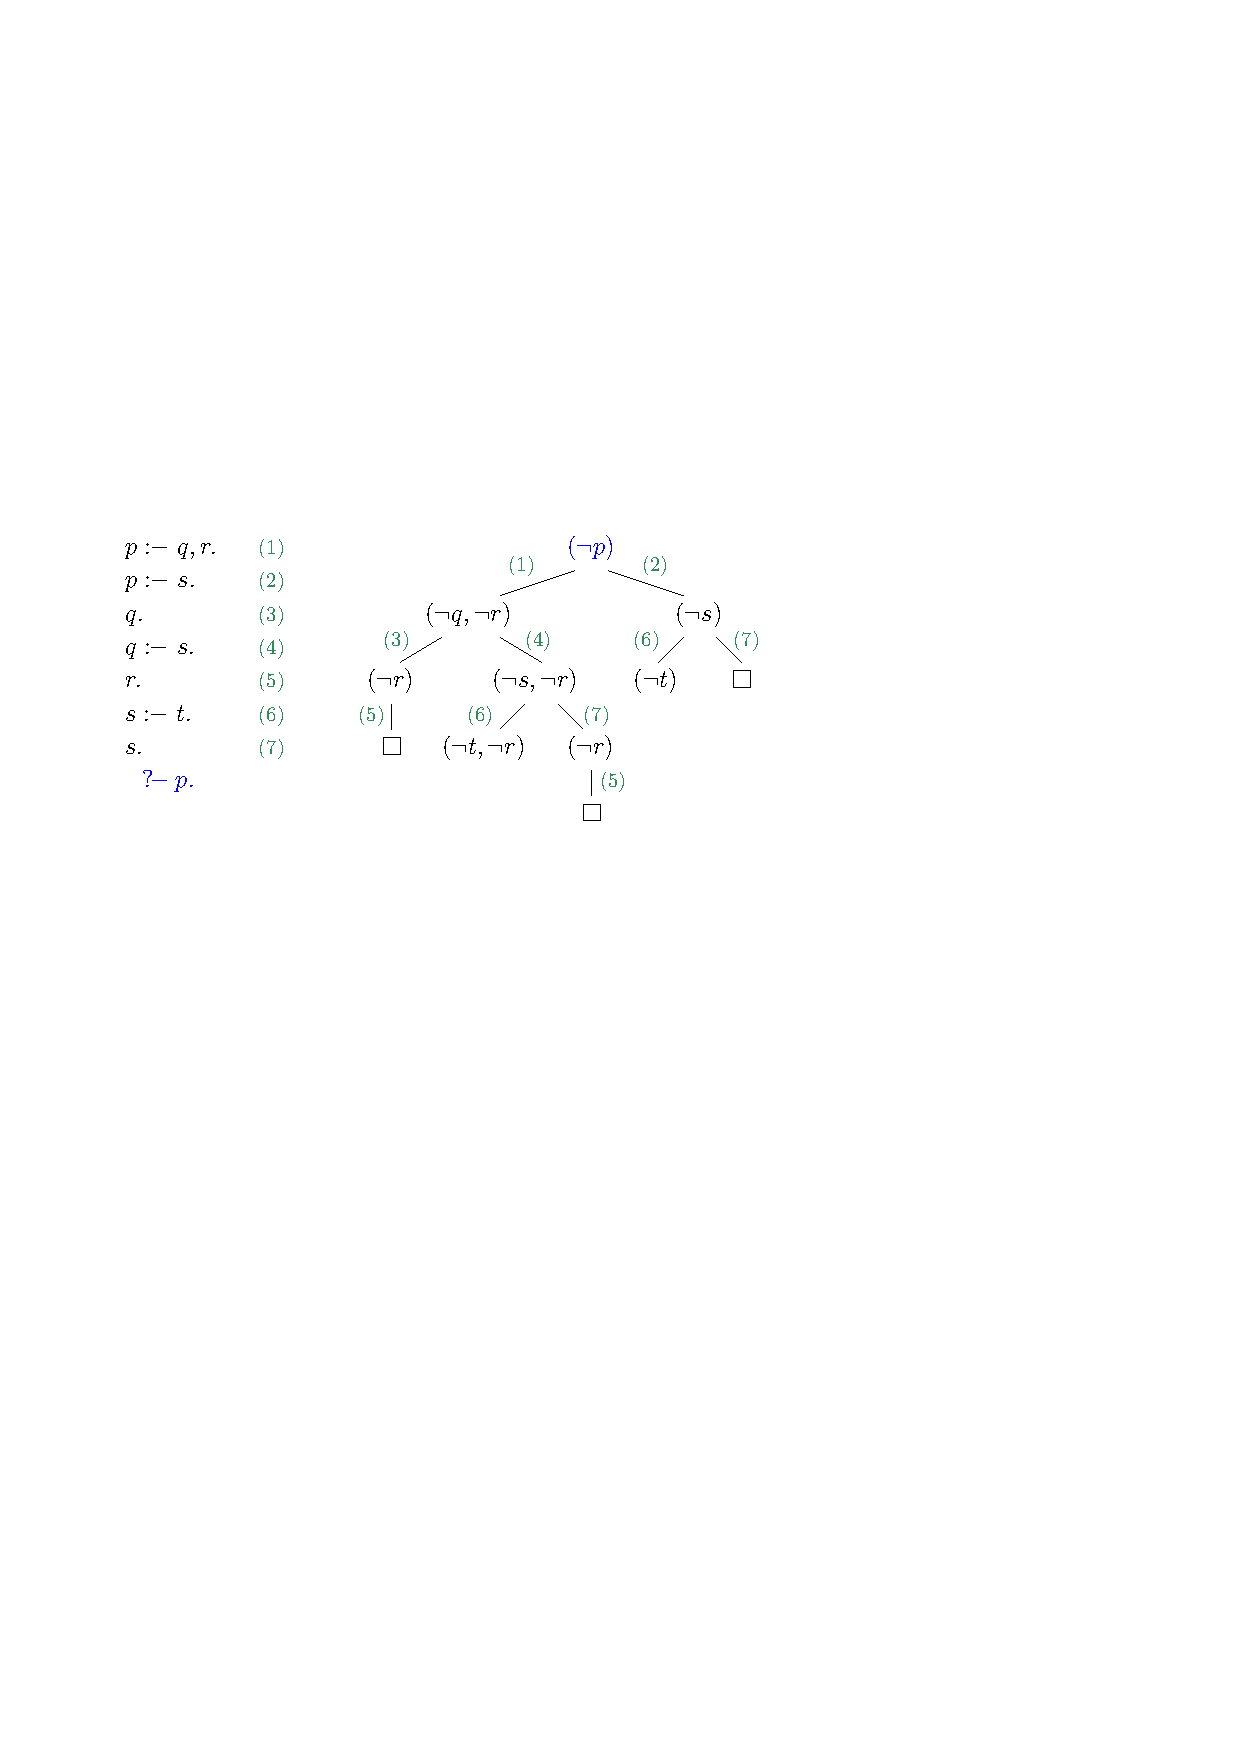
\includegraphics[scale=0.9]{files/rezoluceSLDstrom.pdf}}
\smallskip

%{\it Interpret Prologu prochází tímto SLD-stromem.}

%%%%%%%%%%%%%%%%%%%%%%%%%%%%%%%%%%%%%%%%%%%%%%%%%%%%%%5

\subsubsection*{Závěrečné poznámky}

\begin{itemize}
\item Interpret Prologu \myblue{prochází} SLD-strom, způsob není předepsán.

\item Implementace, které používají \myblue{DFS}, nezachovávají úplnost.

\smallskip
\centerline{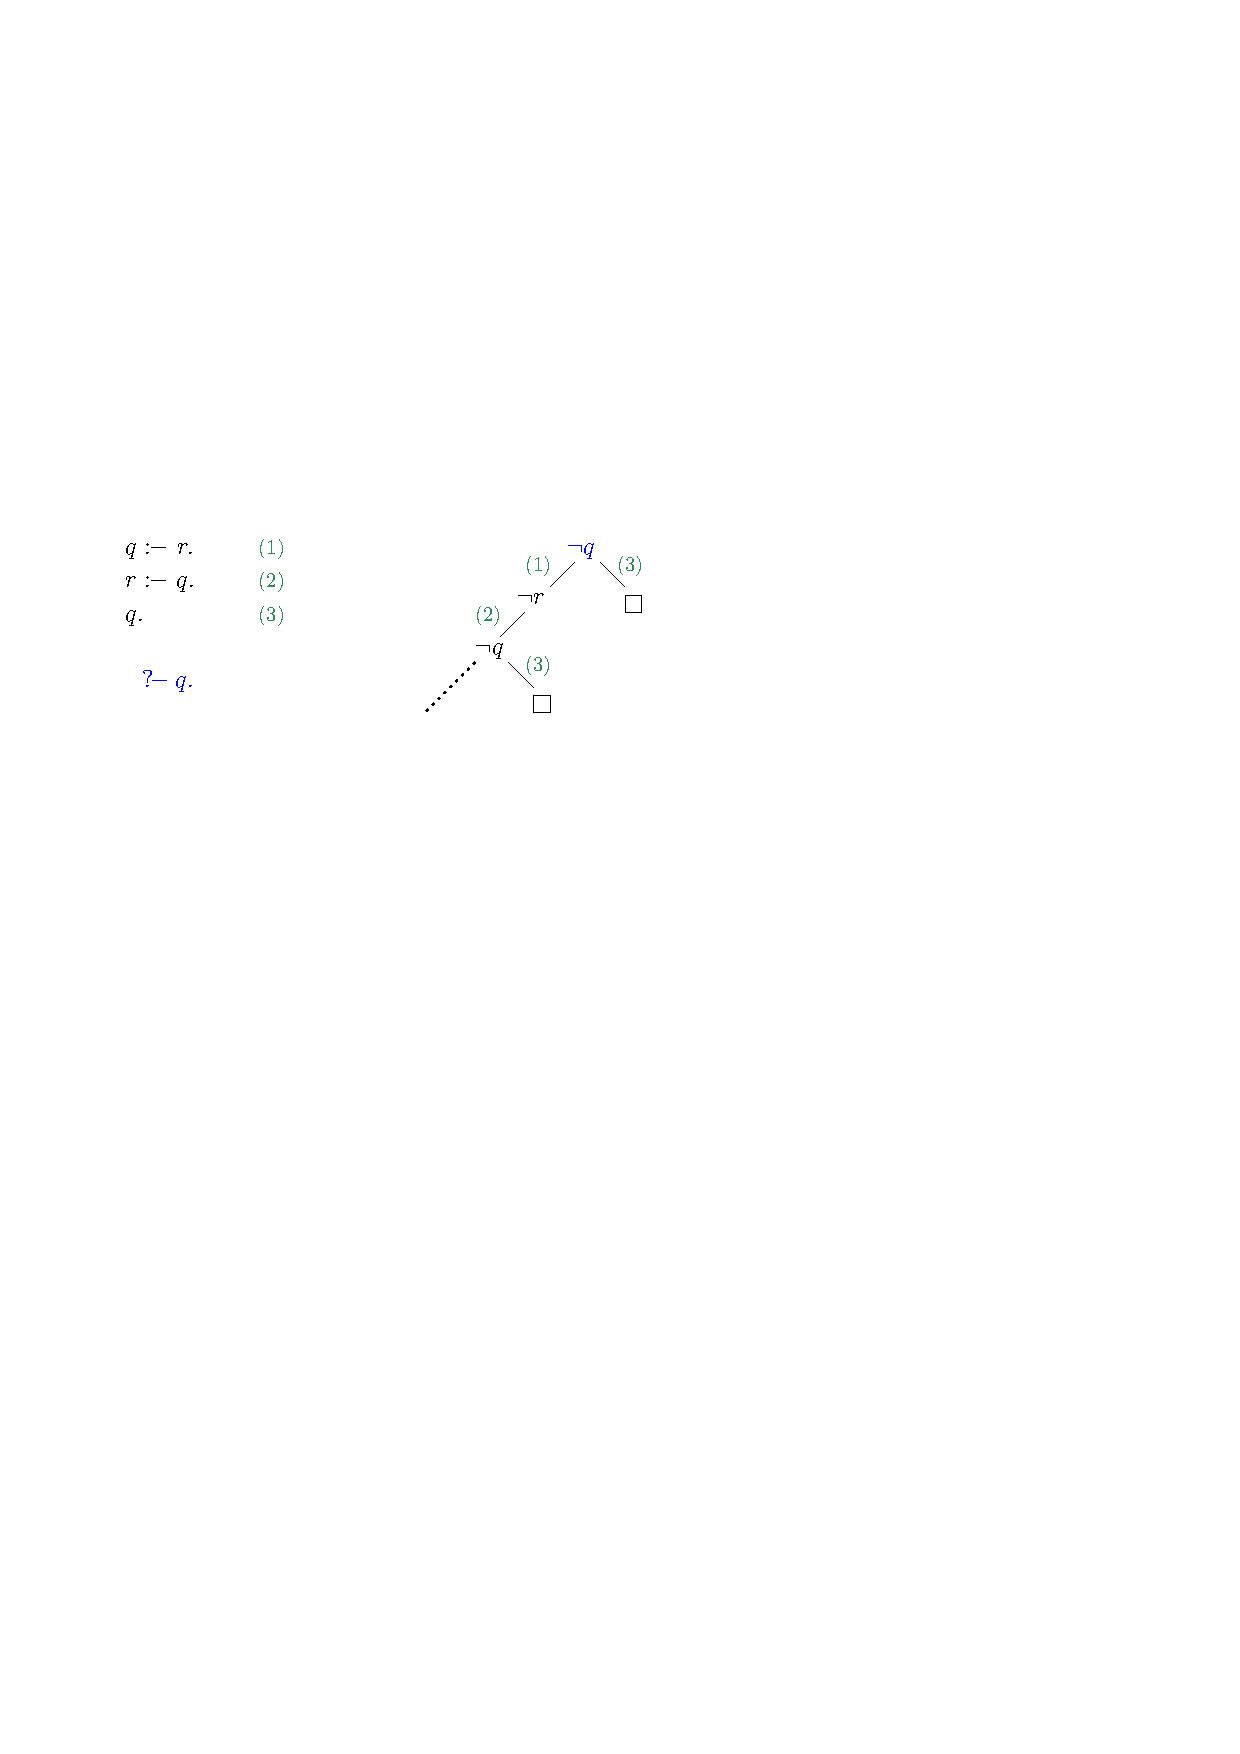
\includegraphics[scale=0.9]{files/rezoluceneuplnost.pdf}}
\smallskip

\item Jistou kontrolu nad prohledáváním poskytuje !, tzv. \myblue{řez}.

\item Při povolení \myblue{negace} nastanou potíže se sémantikou programů.

\item Síla rezoluční metody bude více patrná v predikátové logice.
\end{itemize}

% :from slides
